\documentclass[11pt,a4paper]{article}
\usepackage[margin=20mm]{geometry}
\usepackage[T1]{fontenc}
\usepackage[utf8]{inputenc}
\usepackage{lmodern}
\usepackage{microtype}
\usepackage{graphicx}
\usepackage{booktabs,longtable,tabularx,array}
\usepackage{enumitem}
\usepackage{xcolor}
\usepackage{hyperref}
\usepackage{xurl}
\usepackage{float}
\usepackage{fancyhdr}
\usepackage{titlesec}
\hypersetup{colorlinks=true,linkcolor=blue!55!black,urlcolor=blue!65!black,citecolor=blue!55!black}
\setlength{\parindent}{0pt}
\setlength{\parskip}{5pt}
\setlist[itemize]{topsep=2pt,itemsep=2pt,leftmargin=18pt}
\setlist[enumerate]{topsep=2pt,itemsep=2pt,leftmargin=20pt}
\setlength{\headheight}{14pt}
\emergencystretch=4em
\renewcommand{\_}{\textunderscore\allowbreak}
\sloppy
\pagestyle{fancy}\fancyhf{}\lhead{23CSE455 - Team B5}\rhead{Design Patterns Case Study}\cfoot{\thepage}
\titleformat{\section}{\Large\bfseries}{\thesection}{0.7em}{}
\titleformat{\subsection}{\large\bfseries}{\thesubsection}{0.7em}{}
\begin{document}
\begin{titlepage}
\centering
{\Large 23CSE455 - Design Patterns\par}
\vspace{0.8cm}
{\LARGE\bfseries Design Pattern Identification and Evolution in a Ruby on Rails-Based Travel Planning Application\par}
\vspace{0.8cm}
{\Large Case Study Report - Team B5\par}
\vspace{1.1cm}
\begin{tabular}{lll}
\toprule
Roll number & Student & Batch \\
\midrule
AM.SC.U4CSE23301 & Aakash Choudhary &  CSE D \\
AM.SC.U4CSE23331 & M Tanmayi &  CSE D \\
AM.SC.U4CSE23333 & Manish S D A &  CSE D \\
AM.SC.U4CSE23351 & S Hemarshitha &  CSE D \\
AM.SC.U4CSE23356 & Shreya E R &  CSE D \\
\bottomrule
\end{tabular}
\vfill
\textbf{Application:} DaPlanStan\\
\textbf{Original repository:} \url{https://github.com/GeertClaes/daplanstan}\\
\textbf{Faculty repository:} \url{https://github.com/aswathymohan-amrita/23CSE455_DP_CaseStudy}\\
\textbf{Final verification date:} 11 October 2026
\vfill
{\small Batch confirmed by the team as CSE D.}
\end{titlepage}
\tableofcontents
\newpage

\section{Application and Architecture}
\subsection{Application and source baseline}
DaPlanStan is a self-hosted Ruby on Rails travel-planning application for shared trips. The inspected baseline supports trip creation and membership, email-based booking intake, AI-assisted parsing, itinerary items, map/geocoding workflows, expense tracking, OAuth identity linking, notifications, background jobs and mail delivery.

The source repository is \url{https://github.com/GeertClaes/daplanstan}. The team recorded baseline commit \texttt{da54d9ab8bfc118e99375fdd6c506efb20b66e5b}. The source archive was supplied and first inspected on 8 October 2026. The supplied source ZIP has no \texttt{.git} directory and does not independently establish that archive-to-commit correspondence; the hash is therefore retained as the stated analysis baseline rather than claimed as archive-verified Git metadata.

\textbf{Environment.} The source requires Ruby 3.4.2 and locks Rails 8.1.3. SQLite is used through Active Record. Other important framework/provider boundaries include Turbo/Stimulus, Action Mailbox, Action Mailer, Active Job/Solid Queue, OmniAuth, Anthropic, Geocoder/Nominatim, Pexels and Active Storage. The source license is the O'Saasy License.

\subsection{Architecture and scope}
The architecture was traced from routes, controllers, models, jobs, mailboxes, mailers, initializers and database configuration. The major flow is browser/request to Rails controller, domain model persistence and background jobs; inbound mail routes through Action Mailbox and \texttt{TripMailbox}; parsed confirmations become \texttt{InboxItem} records and may create/link \texttt{TripItem} and \texttt{Expense}; geocoding delegates to the \texttt{Geocodable} concern and Geocoder/Nominatim; OAuth callbacks are coordinated through \texttt{SessionsController} and \texttt{UserIdentity}.

The source does not justify treating \texttt{Trip} as a formally proven DDD aggregate. \texttt{TripItem.kind} represents multiple itinerary kinds rather than separate active Flight/Hotel/Activity domain models. \texttt{Expense} is expense tracking, not verified payment processing. No baseline cancellation workflow was found.

\begin{table}[H]\centering\small
\begin{tabularx}{\linewidth}{p{0.23\linewidth}X}
\toprule
Faculty investigation area & Source-supported finding at the original baseline\\\midrule
Destination management & Trip destination data, cover-image lookup and geocoding/map workflows were inspected.\\
Itinerary management & TripItem creation, import, timeline and map flows were inspected.\\
Hotel/flight/activity booking & Booking-confirmation email intake and parsed itinerary records exist; no active multi-provider booking API integration existed at baseline.\\
Customer management & User, Traveler, Account and TripMember flows were inspected.\\
Payment & Expense records support expense tracking; no verified payment-processing workflow was found.\\
Cancellation & No baseline cancellation-policy or provider-cancellation workflow was found.\\
Notification & Action Mailer/Mail observer logging and trip-scoped Turbo refresh notifications were inspected.\\
\bottomrule
\end{tabularx}
\caption{Coverage of the Part 1 investigation scope specified in the case-study brief.}
\end{table}

\begin{figure}[H]
\centering
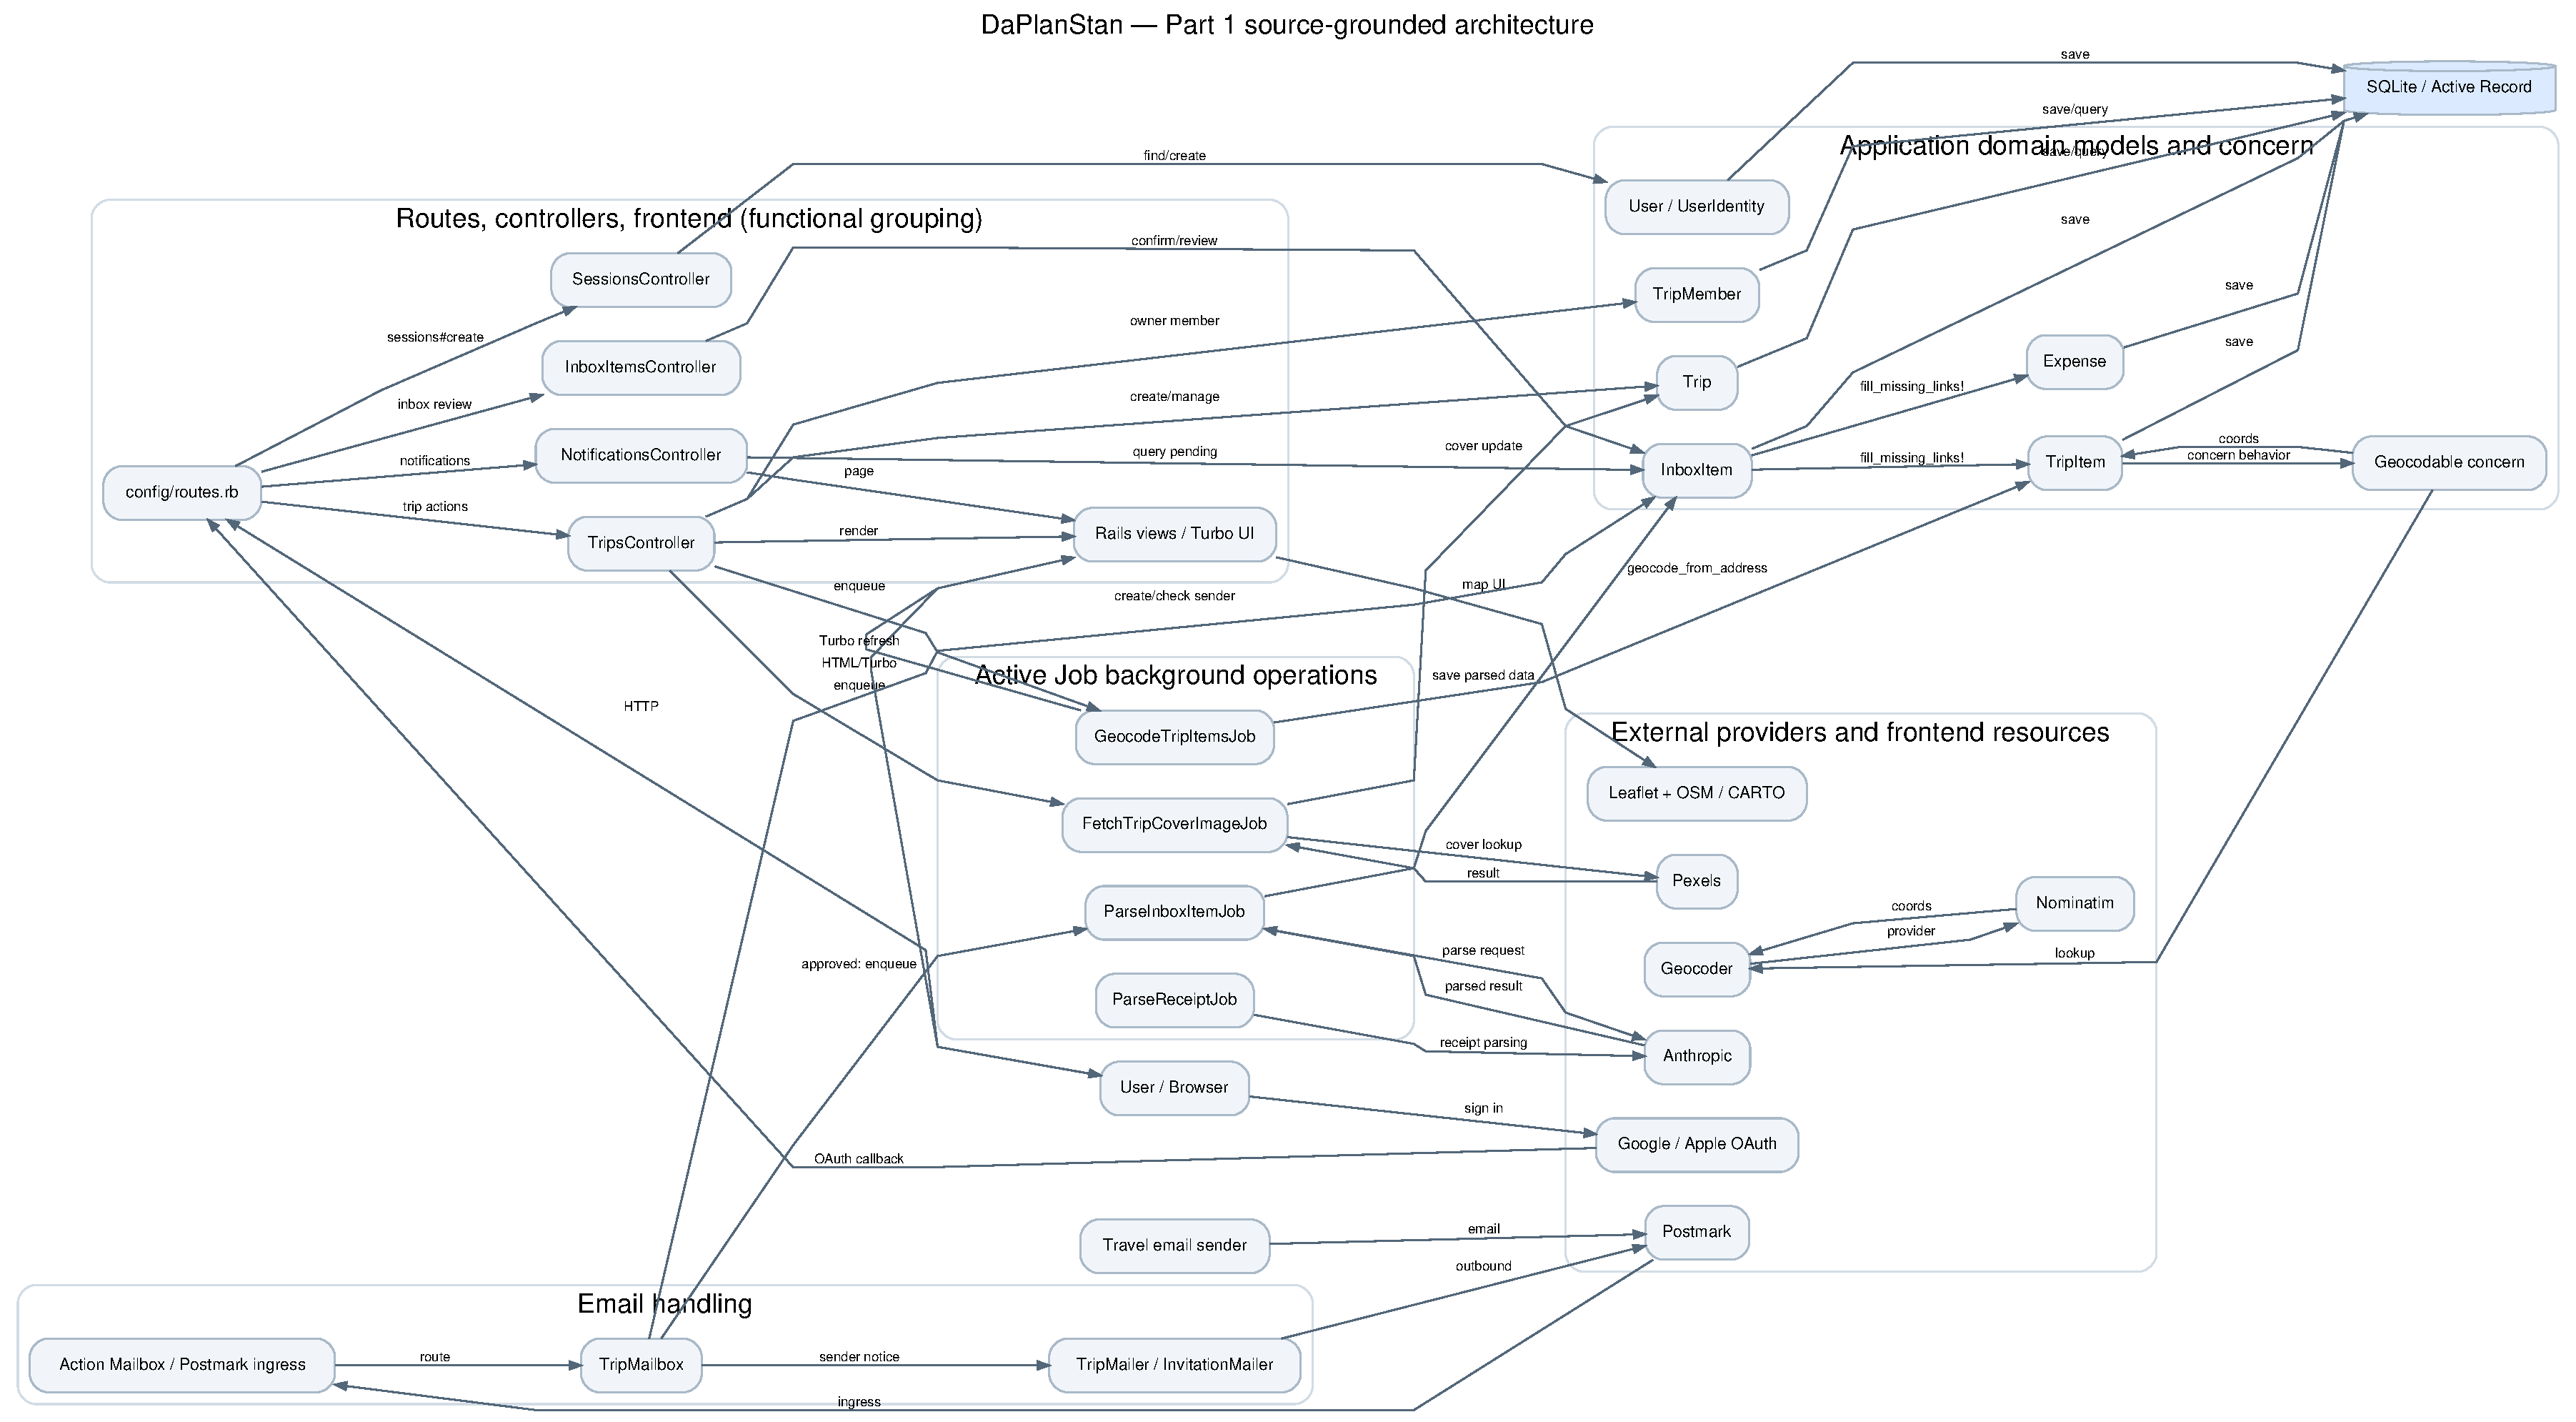
\includegraphics[width=0.98\linewidth]{Part1/pattern_architecture/Part1_DaPlanStan_Architecture.pdf}
\caption{Source-traced DaPlanStan architecture. Editable Mermaid source and SVG are retained under Part1/architecture/.}
\end{figure}

\subsection{Run and final verification}
The original repository README describes normal setup with \texttt{bundle install}, Rails database creation/migration and \texttt{bin/dev}. For final coursework verification, the team installed Ruby 3.4.2 on Windows and resolved native-gem compilation with GNU17 build flags. After environment and test-harness issues were isolated, the cumulative evolved source passed the complete Rails test suite:

\begin{center}\fbox{\textbf{59 runs, 359 assertions, 0 failures, 0 errors, 0 skips}}\end{center}

Rails 8.1.3 with Puma 7.2.0 also booted successfully in the test environment and listened on port 3000 before a clean shutdown. The raw log is \path{data/test_result/rails/rails_test_pass.log}. Historical packaging-time logs that state Rails could not execute are retained as historical records and are superseded by this later successful runtime verification.

\section{Part 1 - Pattern Discovery and Verification}
\subsection{Method}
Pattern candidates were identified only after tracing responsibilities and collaborations in the source. Each candidate was challenged against pattern intent and participant relationships rather than accepted because of a class name, Rails convention or LLM suggestion. Framework-owned roles were explicitly separated from application-owned decisions. Rejected candidates were retained in supporting evidence so the final inventory was not produced by quota seeking.

\subsection{Frozen baseline totals}
The frozen baseline contains \textbf{9 confirmed pattern instances across 3 distinct pattern types}: six Controller (GRASP), one Information Expert (GRASP), and two Observer (GoF).

Following the report template's explicit counting fields, a separate deduplication audit records \textbf{8 concrete participant classes implementing the variable pattern roles}, \textbf{76 distinct mapped participant symbols} (classes, framework interfaces, functions/methods and mapped view/runtime symbols), \textbf{5 rejected candidates}, and \textbf{0 uncertain candidates}. The 76-symbol count is generated from the final P01--P09 participant mappings and is reproducible at \path{Part1/evidence/participant_symbol_audit.csv}; the 8 concrete variable-role classes are listed at \path{Part1/evidence/concrete_participant_class_audit.csv}. Rejected candidates and reasons are preserved at \path{Part1/evidence/rejected_candidates.md}.

\begin{table}[H]\centering
\begin{tabular}{lrr}\toprule
Pattern type & Instances & Category\\\midrule
Controller (GRASP) & 6 & GRASP responsibility assignment\\
Information Expert (GRASP) & 1 & GRASP responsibility assignment\\
Observer (GoF) & 2 & Behavioral\\\bottomrule
\end{tabular}
\caption{Frozen baseline pattern counts.}
\end{table}

\begin{table}[H]\centering
\begin{tabular}{lr}\toprule
Report-template baseline measure & Count\\\midrule
Confirmed pattern types & 3\\
Confirmed pattern instances & 9\\
Concrete participant classes (variable roles; deduplicated) & 8\\
Unique mapped participant symbols & 76\\
Rejected candidates & 5\\
Uncertain candidates & 0\\\bottomrule
\end{tabular}
\caption{Additional baseline totals required by the faculty report template.}
\end{table}

\subsection{Baseline pattern inventory}
\begin{longtable}{p{0.07\linewidth}p{0.18\linewidth}p{0.44\linewidth}p{0.22\linewidth}}
\toprule ID & Pattern & Collaboration & Concrete variable-role class\\\midrule\endfirsthead
\toprule ID & Pattern & Collaboration & Concrete variable-role class\\\midrule\endhead
P01 & Information Expert & Parsed Email to Trip Record Linking & InboxItem\\
P02 & Controller & Inbound Travel Email Intake Coordination & TripMailbox\\
P03 & Controller & Trip Creation Coordination & TripsController\\
P04 & Controller & Trip Membership Management Coordination & TripMembersController\\
P05 & Controller & Bulk Itinerary Import Coordination & TripItemsController\\
P06 & Controller & OAuth Sign-in and Identity Linking Coordination & SessionsController\\
P07 & Controller & Account Traveler Enrollment Coordination & TravelersController\\
P08 & Observer & Outbound Mail Delivery Logging & MailLogger\\
P09 & Observer & Trip-Scoped Turbo Refresh Notifications & Framework-mediated subscriber; no additional application concrete class counted\\
\bottomrule
\end{longtable}

Rejected/uncertain candidates include geocoding as Template Method/Strategy/Adapter, timeline-map Observer, and Beta Invite eligibility as Information Expert. These were rejected because the inspected application interactions did not establish the required pattern collaboration. P08 and P09 explicitly rely in part on framework contracts, which is recorded in their evidence rather than hidden.

\subsection{Evidence records for the nine instances}
The following records summarize the exact participant and location text preserved in the canonical baseline dataset. Full machine-readable records are in \path{data/patterns.csv} and editable/rendered UML is in \path{Part1/architecture/baseline_pattern_uml/}.

\subsubsection*{P01 - Parsed Email to Trip Record Linking}
\textbf{Pattern/category:} Information Expert (GRASP); GRASP - Responsibility Assignment.\par
\textbf{Participant mapping:} Application: InboxItem\#parsed\_data and \#parsed\_data= = stored extraction interface; InboxItem\#confirm\_and\_create\_items! = confirmation and shortlist processing; InboxItem\#fill\_missing\_links! = Information Expert responsible for matching and linking records; InboxItem\#build\_expense = conditional expense creation; InboxItemsController\#update = requesting client; Trip = parent domain context; TripItem = itinerary record; Expense = expense record; TripMember and Traveler = membership and payer lookup; User = reviewing user. Framework: Active Record = associations and persistence.\par
\textbf{Source locations:} \nolinkurl{app/models/inbox_item.rb:19-25,34-58,67-187,191-207; app/controllers/inbox_items_controller.rb:16-35; app/models/trip.rb:4-12; app/models/trip_item.rb:1-28; app/models/expense.rb:1-28; app/models/trip_member.rb:1-6; app/models/traveler.rb:1-8}\par
\textbf{Intent/evidence:} InboxItem holds parsed travel-email data and is assigned responsibility for interpreting it to match or create TripItem records and conditionally create linked Expense records. InboxItemsController delegates confirmation and relinking to InboxItem.\par
\subsubsection*{P02 - Inbound Travel Email Intake Coordination}
\textbf{Pattern/category:} Controller (GRASP); GRASP - Responsibility Assignment.\par
\textbf{Participant mapping:} Application: ApplicationMailbox = inbound routing declaration; TripMailbox\#process = system-event coordinator; TripMailbox\#extract\_text\_body and \#extract\_html\_body = message-content extraction; TripMailbox\#notify\_owners\_of\_pending\_sender = owner-notification coordination; Trip = recipient-address destination; ApprovedSender = sender-approval record; TripMember and Traveler and User = membership and sender-identity checks; InboxItem = persisted incoming message; ParseInboxItemJob\#perform = delegated parsing operation; TripMailer\#pending\_sender\_notification = delegated notification construction. Framework: Action Mailbox = message routing and processing lifecycle; Active Record = persistence; Active Job = background execution; Action Mailer = notification delivery infrastructure. Provider: Anthropic = subsequent AI extraction through ParseInboxItemJob.\par
\textbf{Source locations:} \nolinkurl{app/mailboxes/application_mailbox.rb:1-3; app/mailboxes/trip_mailbox.rb:2-31,35-60; app/models/trip.rb:4-19; app/models/approved_sender.rb:1-6; app/models/inbox_item.rb:1-17; app/models/trip_member.rb:1-6; app/jobs/parse_inbox_item_job.rb:99-112,127-139; app/mailers/trip_mailer.rb:2-10}\par
\textbf{Intent/evidence:} TripMailbox\#process coordinates the incoming-email event by identifying the destination Trip through its inbound address and checking sender eligibility. It creates an InboxItem and delegates approved messages to parsing or unapproved messages to owner notification.\par
\subsubsection*{P03 - Trip Creation Coordination}
\textbf{Pattern/category:} Controller (GRASP); GRASP - Responsibility Assignment.\par
\textbf{Participant mapping:} Application: TripsController\#create = system-event coordinator; ApplicationController\#current\_user and \#current\_account = authenticated context; Trip = new domain object with validation and inbound-address generation; Trip\#generate\_inbound\_email and \#build\_inbound\_email = address-generation operations; Account\#owner\_traveler = owner-traveler lookup; Traveler = selected account participant; TripMember = initial owner-role membership; FetchTripCoverImageJob\#perform = delegated cover-image retrieval. Framework: Rails routing and Active Record = request handling and persistence; Active Job = job execution. Provider: Pexels = external image search.\par
\textbf{Source locations:} \nolinkurl{app/controllers/trips_controller.rb:35-48; app/controllers/application_controller.rb:14-20; app/models/trip.rb:4-19,31-37; app/models/account.rb:9-11; app/models/traveler.rb:1-8; app/models/trip_member.rb:1-6; app/jobs/fetch_trip_cover_image_job.rb:4-32; config/routes.rb:21}\par
\textbf{Intent/evidence:} TripsController\#create coordinates the trip-creation event by saving the new Trip and creating its initial owner-role TripMember through Account\#owner\_traveler. It then delegates cover-image retrieval to FetchTripCoverImageJob.\par
\subsubsection*{P04 - Trip Membership Management Coordination}
\textbf{Pattern/category:} Controller (GRASP); GRASP - Responsibility Assignment.\par
\textbf{Participant mapping:} Application: TripMembersController\#create and \#destroy = membership-event handlers; TripMembersController\#set\_trip = trip resolution; TripMembersController\#require\_owner\_or\_planner = authorization; TripMembersController\#add\_traveler = duplicate checking and membership creation; TripMembersController\#resolve\_and\_add\_by\_email = traveler resolution and invitation coordination; ApplicationController\#current\_member\_for = acting-user membership lookup; Trip and Account = trip and account context; Traveler and User = participant identity; TripMember = role-bearing membership; InvitationMailer\#invite\_to\_trip = invitation construction. Framework: Rails routing and Active Record = request handling and association persistence; Action Mailer and Active Job = mail infrastructure.\par
\textbf{Source locations:} \nolinkurl{app/controllers/trip_members_controller.rb:6-22,26-65; app/controllers/application_controller.rb:22-25; app/models/trip.rb:4-12; app/models/account.rb:1-11; app/models/traveler.rb:1-8; app/models/user.rb:11-17; app/models/trip_member.rb:1-6; app/mailers/invitation_mailer.rb:8-13; config/routes.rb:40}\par
\textbf{Intent/evidence:} TripMembersController coordinates addition and removal of members in an existing Trip. It checks owner or planner authorization and resolves account travelers before creating contributor-role memberships or removing permitted memberships. Invitation delivery is delegated to InvitationMailer.\par
\subsubsection*{P05 - Bulk Itinerary Import Coordination}
\textbf{Pattern/category:} Controller (GRASP); GRASP - Responsibility Assignment.\par
\textbf{Participant mapping:} Application: TripItemsController\#import = import-event coordinator for preview and confirmation; TripItemsController\#bulk\_create\_items = batch matching and persistence coordination; TripItemsController\#parse\_import\_time = imported date-time parsing; Trip = destination context; TripItem = existing or newly imported itinerary record; Geocodable\#geocoded? = coordinate-completeness check; GeocodeTripItemsJob\#perform = delegated geocoding; import.html.erb = preview and confirmation interface. Framework: Rails routing and Active Record = queries and persistence; Active Job = deferred execution.\par
\textbf{Source locations:} \nolinkurl{app/controllers/trip_items_controller.rb:31-58,128-179; app/models/trip.rb:4-12; app/models/trip_item.rb:1-28; app/models/concerns/geocodable.rb:9-11; app/jobs/geocode_trip_items_job.rb:4-21; app/views/trip_items/import.html.erb:93-106; config/routes.rb:30-34}\par
\textbf{Intent/evidence:} TripItemsController\#import coordinates JSON preview and confirmed batch import as one use case. Its bulk\_create\_items operation checks names and duplicates and creates or updates itinerary ideas before scheduling GeocodeTripItemsJob for missing coordinates.\par
\subsubsection*{P06 - OAuth Sign-in and Identity Linking Coordination}
\textbf{Pattern/category:} Controller (GRASP); GRASP - Responsibility Assignment.\par
\textbf{Participant mapping:} Application: SessionsController\#create = post-authentication system-event coordinator; SessionsController\#provision\_account\_or\_gate = account-eligibility coordination; SessionsController\#create\_account\_for = account and initial-traveler creation; UserIdentity = external provider identity record; User = local authenticated identity; Traveler\#accept! = pending invitation association; Account = user-owned account; Invite\#usable? and \#email\_matches? = invite-eligibility predicates; ApplicationController\#current\_user = session identity lookup; OmniAuth initializer = provider configuration. Framework: OmniAuth and provider integrations = OAuth processing and normalized authentication data; Rails sessions and Active Record = local session and persistence.\par
\textbf{Source locations:} \nolinkurl{app/controllers/sessions_controller.rb:4-41,54-81; app/models/user_identity.rb:1-8; app/models/user.rb:11-22; app/models/traveler.rb:26-28; app/models/account.rb:1-11; app/models/invite.rb:12-18; app/controllers/application_controller.rb:14-16; config/initializers/omniauth.rb:1-16; config/routes.rb:12-14}\par
\textbf{Intent/evidence:} SessionsController\#create coordinates post-OAuth identity handling by finding a UserIdentity through provider and UID or resolving a User by email. It creates missing identity links and establishes the session before accepting pending travelers and applying account-provisioning or invitation rules.\par
\subsubsection*{P07 - Account Traveler Enrollment Coordination}
\textbf{Pattern/category:} Controller (GRASP); GRASP - Responsibility Assignment.\par
\textbf{Participant mapping:} Application: TravelersController\#create = account-enrollment system-event coordinator; TravelersController\#set\_account = account-owner access control; Account = account-scoped traveler context; Traveler = new account participant; User = registered identity lookup; InvitationMailer\#invite = account invitation construction; settings/show.html.erb = enrollment interface. Framework: Rails routing and Active Record = request handling and persistence; Action Mailer and Active Job = invitation delivery infrastructure.\par
\textbf{Source locations:} \nolinkurl{app/controllers/travelers_controller.rb:5-35,54-56; app/models/account.rb:1-11; app/models/traveler.rb:1-8,18-28; app/models/user.rb:11-22; app/mailers/invitation_mailer.rb:2-6; app/views/settings/show.html.erb:114-127; config/routes.rb:48-50}\par
\textbf{Intent/evidence:} TravelersController\#create coordinates account-level traveler enrollment by validating supplied identity information and checking existing participants. It creates name-only or email-based Traveler records and links registered Users or requests invitations when applicable. This does not itself establish TripMember membership.\par
\subsubsection*{P08 - Outbound Mail Delivery Logging}
\textbf{Pattern/category:} Observer (GoF); GoF - Behavioral (framework-mediated).\par
\textbf{Participant mapping:} Application: MailLogger = concrete observer; MailLogger.delivered\_email(message) = notification callback; ActionMailer::Base.register\_observer(MailLogger) = application registration call; InvitationMailer\#invite and \#invite\_to\_trip = mail-producing collaborators; TripMailer\#pending\_sender\_notification = mail-producing collaborator. Framework: ActionMailer::Base.register\_observer = observer registration interface; Mail gem = publisher and observer registry and notification dispatch; Action Mailer = mail lifecycle. Provider: Postmark = external delivery transport and not an Observer participant.\par
\textbf{Source locations:} \nolinkurl{config/initializers/mail_logger.rb:1-7; app/mailers/invitation_mailer.rb:2-13; app/mailers/trip_mailer.rb:2-10; app/mailers/application_mailer.rb:1-5; Gemfile.lock:19,185}\par
\textbf{Intent/evidence:} DaPlanStan defines MailLogger.delivered\_email and explicitly registers MailLogger through ActionMailer::Base.register\_observer. The Mail framework invokes the registered concrete observer during the delivery lifecycle so individual mailers do not directly call the logger.\par
\subsubsection*{P09 - Trip-Scoped Turbo Refresh Notifications}
\textbf{Pattern/category:} Observer (GoF); GoF - Behavioral (framework-mediated).\par
\textbf{Participant mapping:} Application: InboxItem = model publication source through broadcasts\_refreshes\_to :trip; GeocodeTripItemsJob\#perform = explicit broadcast source through Turbo::StreamsChannel.broadcast\_refresh\_to(trip); trips/show.html.erb = trip-page subscription and refresh configuration; inbox\_items/index.html.erb = inbox-page subscription. Framework: Turbo::Broadcastable = model-triggered broadcast implementation; Turbo::StreamsChannel = trip-stream subscription and publication channel; Turbo::Streams::Broadcasts = refresh broadcast implementation; Action Cable = stream delivery infrastructure; Turbo browser runtime = concrete stream subscriber and refresh reaction.\par
\textbf{Source locations:} \nolinkurl{app/models/inbox_item.rb:1-5; app/jobs/geocode_trip_items_job.rb:4-21; app/views/trips/show.html.erb:2-9; app/views/inbox_items/index.html.erb:1; Gemfile.lock:424; Turbo Rails 2.0.23: app/models/concerns/turbo/broadcastable.rb; Turbo Rails 2.0.23: app/channels/turbo/streams_channel.rb; Turbo Rails 2.0.23: app/channels/turbo/streams/broadcasts.rb}\par
\textbf{Intent/evidence:} InboxItem changes and GeocodeTripItemsJob completion request refresh broadcasts for a Trip. The trip show and inbox index pages subscribe through turbo\_stream\_from @trip. Turbo Rails and Action Cable implement subscription and notification delivery as one shared trip-scoped Observer collaboration.\par

\subsection{Per-instance origin, diagram and human verification}
Each P01--P09 record above is source-backed. The table below supplies the report-template origin/verification fields without changing the frozen classifications. Human-verification labels are copied from the consolidated team verification sheet; reviewer display aliases are mapped to official team names in \path{data/test_result/human_verification/REVIEWER_NAME_MAP.md}.

\begin{longtable}{p{0.07\linewidth}p{0.35\linewidth}p{0.20\linewidth}p{0.27\linewidth}}
\toprule ID & Origin & Human verification & Diagram\\\midrule\endfirsthead
\toprule ID & Origin & Human verification & Diagram\\\midrule\endhead
P01 & Application responsibility; Active Record persistence framework & S Hemarshitha - verified & \path{Part1/pattern_architecture/baseline_pattern_uml/svg/P01_Parsed_Email_to_Trip_Record_Linking.svg}\\
P02 & Application mailbox coordinator with Rails/mail/job framework support & Manish S D A - verified & \path{Part1/pattern_architecture/baseline_pattern_uml/svg/P02_Inbound_Travel_Email_Intake_Coordination.svg}\\
P03 & Application Rails controller with persistence/job/provider collaborators & Manish S D A - verified & \path{Part1/pattern_architecture/baseline_pattern_uml/svg/P03_Trip_Creation_Coordination.svg}\\
P04 & Application Rails controller with membership/mailer collaborators & Manish S D A - verified & \path{Part1/pattern_architecture/baseline_pattern_uml/svg/P04_Trip_Membership_Management_Coordination.svg}\\
P05 & Application Rails controller with persistence/geocoding collaborators & Aakash Choudhary - verified & \path{Part1/pattern_architecture/baseline_pattern_uml/svg/P05_Bulk_Itinerary_Import_Coordination.svg}\\
P06 & Application Rails controller with OmniAuth framework/provider boundary & S Hemarshitha - verified & \path{Part1/pattern_architecture/baseline_pattern_uml/svg/P06_OAuth_Signin_and_Identity_Linking_Coordination.svg}\\
P07 & Application Rails controller with mail delivery infrastructure & M Tanmayi - verified & \path{Part1/pattern_architecture/baseline_pattern_uml/svg/P07_Account_Traveler_Enrollment_Coordination.svg}\\
P08 & Application concrete observer registered through Action Mailer/Mail & Shreya E R - verified & \path{Part1/pattern_architecture/baseline_pattern_uml/svg/P08_Outbound_Mail_Delivery_Logging.svg}\\
P09 & Application broadcast/subscription declarations with Turbo/Action Cable framework delivery & Manish S D A - verified & \path{Part1/pattern_architecture/baseline_pattern_uml/svg/P09_Trip_Scoped_Turbo_Refresh_Notifications.svg}\\
\bottomrule
\end{longtable}

\section{Part 2 - Software Evolution and Refactoring}
Three cumulative realistic changes from the assigned case study were implemented in order. The original baseline remains frozen; each AFTER snapshot is preserved either directly or as an exact input ZIP plus change patch. Evolution status is recorded in \path{data/patterns_evolution.csv}.

\subsection{CH01 - Personalized itinerary generation}
\textbf{Requirement and acceptance criteria.} An authenticated trip owner can enter supported interests, budget, pace and notes; receive at most six validated suggestions; preview without persistence; reject with no write; or accept a signed, trip/user-bound preview that is revalidated and persisted only as itinerary \texttt{idea} items. Generated payloads cannot inject booking/payment/status fields. Existing import behavior and geocoding remain functional.

\textbf{Before/after and source.} BEFORE is \path{data/code/original/daplanstan-main/}. The exact Scenario 1 AFTER source used for the next change is preserved as \path{Part2/code/snapshots/scenario1_personalized_itinerary_AFTER.zip}. The main source diff is \path{Part2/changes/Change1/source.patch} and the full change record is \path{Part2/changes/Change1/SCENARIO1_CHANGE_RECORD.md}.

\textbf{Implementation and tests.} \texttt{ItinerarySuggestionGenerator} validates preferences and suggestions, calls the Anthropic tool contract, and returns a transient proposal. \texttt{TripItemsController} coordinates preview/confirmation and reuses batch persistence. Historical isolated checks recorded \textbf{6 runs / 20 assertions}; the Rails environment was then unavailable, so no historical Rails pass is invented. The final cumulative source was later included in the all-green Rails verification.

\textbf{Pattern effects and refactoring.} P05 Bulk Itinerary Import Coordination is \textbf{modified}; S1-N01 Personalized Itinerary Generation Coordination is \textbf{newly introduced} as Controller (GRASP). The refactoring replaces global callback manipulation with instance-scoped deferred geocoding. Snapshot total: \textbf{10 instances / 3 types}.

\subsection{CH02 - Multiple booking providers}
\textbf{Requirement and acceptance criteria.} Two differently shaped provider inputs must be selectable by an authenticated trip owner and normalized to one application-facing offer contract. Provider-specific fields and sample amounts are re-resolved from server-owned local data rather than trusted from the browser. Adding a sample offer creates only an itinerary \texttt{idea}; it must not perform a real reservation, payment or confirmation.

\textbf{Before/after and source.} BEFORE is the Scenario 1 ZIP above. The exact Scenario 2 AFTER input for CH03 is preserved at \path{Part2/code/snapshots/scenario2_multiple_booking_providers_AFTER.zip}. Diff and source verification are \path{Part2/changes/Change2/source.patch} and \path{Part2/changes/Change2/Scenario2_AFTER_source_verification.md}.

\textbf{Implementation and tests.} \texttt{BookingProviders::AtlasAdapter} and \texttt{BeaconAdapter} normalize distinct fixture schemas through the Registry; \texttt{BookingOptionsController} coordinates option display and sample-item creation. Isolated provider checks recorded \textbf{10 runs / 67 assertions}. Final Rails execution later found one duplicate-marker lookup defect, which was corrected to exact substring matching before the final all-green run.

\textbf{Pattern effects.} S2-N01 Multiple Booking Provider Normalization is one \textbf{Adapter (GoF)} collaboration containing both concrete adapters; S2-N02 Multiple Booking Provider Option Coordination is one new \textbf{Controller (GRASP)}. Snapshot total: \textbf{12 instances / 4 types}. Two provider adapters are not counted as two Adapter pattern instances.

\subsection{CH03 - Different cancellation policies}
\textbf{Requirement and acceptance criteria.} Eligible confirmed email-linked TripItems can receive deterministic hypothetical cancellation quotes under Flexible, Moderate or Strict policies. Exact 72-hour and 24-hour boundaries are fixed; unknown policies and ineligible/tampered data are rejected; server-loaded amount/start/currency are used; money uses BigDecimal half-up rounding; GET/POST are quote-only and perform no cancellation, refund, booking-state write or external provider call.

\textbf{Before/after and source.} BEFORE is the Scenario 2 ZIP. The final corrected cumulative source is stored directly at \path{Part2/code/final/}. Diff/source verification are \path{Part2/changes/Change3/source.patch} and \path{Part2/changes/Change3/Scenario3_AFTER_source_verification.md}.

\textbf{Implementation and tests.} \texttt{CancellationPolicies::QuoteEvaluator} selects a whitelisted policy and computes fee/refund; the three policies implement one fee-rate protocol; \texttt{CancellationQuotesController} coordinates owner-authorized quotes. Isolated checks recorded \textbf{10 runs / 45 assertions}. The final cumulative Rails suite then passed \textbf{59 runs / 359 assertions / 0 failures / 0 errors / 0 skips}.

\textbf{Pattern effects.} S3-N01 Cancellation Policy Evaluation is one \textbf{Strategy (GoF)} collaboration containing three concrete strategies; S3-N02 Cancellation Quote Coordination is one new \textbf{Controller (GRASP)}. Final total: \textbf{14 instances / 5 types}.

\subsection{Updated counts and before/after metrics}
The same LOC rule is applied to each snapshot: include \texttt{app/**/*.rb} and \texttt{config/routes.rb}; exclude blank/comment-only lines, tests, views, generated database files, documentation and evidence scripts. The reproducible method is \path{Part2/evidence/EVOLUTION_METRICS_METHOD.md}.

\begin{table}[H]\centering\small
\begin{tabularx}{\linewidth}{lrrrrX}
\toprule
Snapshot & Source LOC & Instances & Types & Concrete variable-role classes & Actual execution evidence\\\midrule
Baseline & 1797 & 9 & 3 & 8 & Supplied baseline had no application test suite\\
CH01 & 2011 & 10 & 3 & 8 & 6 runs / 20 assertions isolated; historical Rails blocked\\
CH02 & 2197 & 12 & 4 & 11 & 10 runs / 67 assertions isolated; historical Rails blocked\\
CH03 final & 2332 & 14 & 5 & 15 & 10 runs / 45 assertions isolated; final cumulative Rails 59/359, 0 failures/errors\\
\bottomrule
\end{tabularx}
\caption{Evolution metrics using one fixed measurement scope.}
\end{table}

The increase in LOC is reported as descriptive evidence only. It does not by itself prove better design. Benefits instead come from explicit separation of new variability: generated-itinerary coordination, provider normalization and interchangeable cancellation rules. Trade-offs include more application code, fictional provider/cancellation assumptions, and no live provider/payment/cancellation integration.

\subsection{Runtime-discovered corrections and diagrams}
Final Rails runtime verification exposed one Scenario 2 duplicate-detection query defect and two Scenario 1 Minitest stub-compatibility issues. These corrections are documented at \path{data/test_result/rails/RUNTIME_ISSUE_RESOLUTION.md}. The final source at \path{Part2/code/final/} contains the corrected query and compatible test stubs. Editable DOT and rendered SVG diagrams for S1-N01, S2-N01, S2-N02, S3-N01 and S3-N02 are in \path{Part2/diagrams/}.

\section{Part 3 - Cross-Language Comparison}
The short case-study brief requested two significant patterns. The later detailed faculty CSV instruction required one representative confirmed instance for each detected pattern type. The team followed the stricter requirement: one representative for all five confirmed types, each implemented in Java, Python, JavaScript and C++ using the same language-neutral fixtures and expected outputs.

\begin{table}[H]\centering\small
\begin{tabularx}{\linewidth}{lX}\toprule
Pattern & Representative source collaboration\\\midrule
Controller & Trip Creation Coordination (P03)\\
Information Expert & Parsed Email to Trip Record Linking (P01)\\
Observer & Outbound Mail Delivery Logging (P08)\\
Adapter & Multiple Booking Provider Normalization (S2-N01)\\
Strategy & Cancellation Policy Evaluation (S3-N01)\\\bottomrule
\end{tabularx}
\caption{Representative source-grounded pattern problems.}
\end{table}

The result is \textbf{20 implementations}: 5 pattern types multiplied by 4 languages. Recorded shared-fixture results are Strategy 60/60, Observer 28/28, Controller 32/32, Information Expert 32/32 and Adapter 40/40, for \textbf{192/192 passing cases}. The exact 20-row faculty dataset is \path{data/cross_language.csv}.

\subsection{Static and dynamic comparison}
\begin{longtable}{lrrrrrrrr}
\toprule & \multicolumn{4}{c}{Source LOC} & \multicolumn{4}{c}{Maximum function CC}\\
Pattern & Java & Python & JS & C++ & Java & Python & JS & C++\\\midrule\endfirsthead
\toprule & \multicolumn{4}{c}{Source LOC} & \multicolumn{4}{c}{Maximum function CC}\\
Pattern & Java & Python & JS & C++ & Java & Python & JS & C++\\\midrule\endhead
Strategy & 52 & 54 & 42 & 74 & 12 & 8 & 8 & 15\\
Observer & 47 & 32 & 43 & 60 & 5 & 5 & 5 & 4\\
Controller & 66 & 59 & 55 & 90 & 9 & 10 & 9 & 13\\
Information Expert & 63 & 45 & 38 & 83 & 7 & 7 & 6 & 7\\
Adapter & 120 & 93 & 67 & 141 & 12 & 7 & 8 & 12\\
\bottomrule
\end{longtable}

\begin{table}[H]\centering\small
\begin{tabular}{lrrrr}\toprule
Pattern & Java ms & Python ms & JS ms & C++ ms\\\midrule
Strategy & 91.907 & 839.469 & 30.426 & 2.582\\
Observer & 109.548 & 1133.245 & 43.673 & 2.325\\
Controller & 159.473 & 818.330 & 37.862 & 2.566\\
Information Expert & 75.602 & 819.622 & 36.436 & 4.391\\
Adapter & 71.668 & 852.240 & 35.246 & 2.706\\
\bottomrule
\end{tabular}
\caption{Recorded median fresh-process times from \texttt{data/cross\_language.csv}; these include process/test-harness overhead.}
\end{table}

The implementations use OpenJDK/javac 21.0.12.1, Python 3.13.5, Node.js 22.16.0 and g++ 14.2.0 with C++17. Timing was measured after compilation where applicable, with one warm-up and five measured fresh-process executions on the same machine. Reported medians include process startup/runtime/test-harness overhead, so they are not pure algorithm benchmarks.

Across the fixed examples, Java and C++ use more explicit types/interfaces in several patterns, while Python and JavaScript express equivalent roles more compactly. These LOC and timing observations are descriptive only and do not establish that one language or pattern implementation is universally superior.

\section{LLM Records and Human Verification}
\subsection{LLM records}
The canonical \path{data/llm.csv} contains \textbf{29 provenance-audited interaction records} using exactly the seven required columns: part, model/date, prompt file, input file, output file, evaluation and verification file. The official part names in the final CSV are Part 1 Pattern Discovery, Part 2 Software Evolution and Part 3 Cross-Language Analysis.

The team also supplied authentic full exported ChatGPT conversation PDFs. Per the team's faculty instruction, the PDFs are retained rather than replaced by invented text transcripts:
\begin{itemize}
\item \path{Part1/Part1_prompt.pdf} - official Part 1 pattern-discovery conversation.
\item \path{Part1/llm/Architecture_Chat_ShreyaER.pdf} - application/architecture conversation.
\item \path{Part2/Part2_prompt.pdf} - official Part 2 software-evolution conversation.
\item \path{Part3/llm/part3_prompt.pdf} - official Part 3 cross-language conversation.
\item \path{Part3/llm/Final_Documentation_Chat_MTanmayi.pdf} - final LLM/human-verification/documentation workflow.
\end{itemize}

Historical exact model configurations were not recoverable for the older interactions, so \path{data/llm.csv} says \texttt{cannot confirm} instead of inventing model names. Interaction-level recovered prompt/output material remains under each part's \path{llm/audit/} directory. Historical evaluation wording is preserved as audit-time evidence; later human review is recorded separately.

\subsection{Human verification}
The consolidated human-verification sheet contains \textbf{148 items}: \textbf{143 verified}, \textbf{3 partially verified} and \textbf{2 cannot confirm}, dated 2026-10-11. It is preserved at \path{data/test_result/human_verification/human_verification_final_team.csv} and as the original XLSX companion file. Review assignments were distributed across all five team members; the raw reviewer display names are mapped to official submission names in \path{data/test_result/human_verification/REVIEWER_NAME_MAP.md}.

One cannot-confirm item concerned application setup/boot at the time of human review. Later machine evidence established successful Rails/Puma boot and a full all-green test suite; the historical human sheet is not retroactively rewritten. The other persistent limitation is the inability to prove that the supplied source ZIP is byte-for-byte the stated Git commit because the archive contains no \texttt{.git} metadata.

\section{Findings, Contributions and Limitations}
\subsection{Findings}
The case study shows that source-level pattern classification is more reliable when collaborations are counted by responsibility and interaction rather than by class count. The baseline is dominated by GRASP Controllers because Rails controllers coordinate distinct system events, while the two confirmed Observer cases depend partly on framework notification contracts. Evolution adds Adapter and Strategy only when new variability genuinely appears: incompatible provider schemas in Scenario 2 and interchangeable cancellation policies in Scenario 3.

The cumulative inventory grows from 9 instances/3 types to 14 instances/5 types without retroactively relabeling the baseline. Cross-language implementations preserve the same pattern problems and participant responsibilities across four languages, while syntax, type systems, abstraction mechanisms and process overhead differ.

\subsection{Student contributions}
The team confirmed the following primary workstream ownership. All members also participated in the consolidated human verification/final review recorded in the verification sheet.

\begin{longtable}{p{0.23\linewidth}p{0.25\linewidth}p{0.42\linewidth}}
\toprule Roll number & Student & Recorded contribution\\\midrule\endfirsthead
\toprule Roll number & Student & Recorded contribution\\\midrule\endhead
AM.SC.U4CSE23301 & Aakash Choudhary & Official Part 2 - Software Evolution and Refactoring\\
AM.SC.U4CSE23331 & M Tanmayi & LLM records, Human Verification and Final Documentation\\
AM.SC.U4CSE23333 & Manish S D A & Official Part 3 - Cross-Language Analysis\\
AM.SC.U4CSE23351 & S Hemarshitha & Official Part 1 - Pattern Discovery and Verification\\
AM.SC.U4CSE23356 & Shreya E R & Application Understanding and Framework Architecture\\\bottomrule
\end{longtable}

\subsection{Limitations}
\begin{itemize}
\item The baseline archive lacks Git metadata; commit correspondence is qualified.
\item No live Anthropic API generation was performed in final manual verification. Scenario 1 is covered by controlled tests, and no API key is included.
\item Scenario 2 uses fictional Atlas/Beacon fixtures and does not perform a real reservation or payment.
\item Scenario 3 is a quote-only demonstration; it does not cancel bookings or issue refunds.
\item Optional VIPS loader warnings occurred on Windows but did not block Rails tests or server boot.
\item Historical LLM model identifiers are unconfirmed and copied/printed outputs are not represented as byte-exact native exports.
\end{itemize}

\section{Team Folder and Datasets}
The final team folder follows the faculty's three official technical parts. Canonical datasets are stored once under \path{data/}; supporting code/evidence is organized under Part1, Part2 and Part3. No top-level Part4 or Part5 submission stage is used.

\begin{itemize}
\item \path{data/patterns.csv} - 9 frozen baseline collaborations.
\item \path{data/pattern_counts.csv} - per-pattern and total counts across four snapshots.
\item \path{data/patterns_evolution.csv} - 45 versioned collaboration rows.
\item \path{data/cross_language.csv} - 20 language/pattern rows.
\item \path{data/llm.csv} - 29 provenance-audited LLM records.
\item \path{data/code/original/} - original application source.
\item \path{data/test_result/} - Rails runtime and human-verification evidence.
\item \path{Part1/pattern_architecture/}, \path{Part1/evidence/}, \path{Part1/llm/} - pattern-discovery support.
\item \path{Part2/code/}, \path{Part2/changes/}, \path{Part2/diagrams/}, \path{Part2/evidence/}, \path{Part2/llm/} - evolution support.
\item \path{Part3/} - five representative pattern problems, four languages each, common fixtures, execution evidence and LLM material.
\item \path{Part3/llm/B5_slide.pdf} - requested presentation PDF.
\end{itemize}

\subsection{GitHub team-folder screenshot}
The following screenshot shows the actual B5 team folder after it was pushed to the team's GitHub fork. The repository view visibly contains the required \path{Part1/}, \path{Part2/}, \path{Part3/}, \path{data/}, \path{B5_Report.pdf}, \path{B5_Report.tex}, and \path{README.md} entries.

\begin{figure}[H]
    \centering
    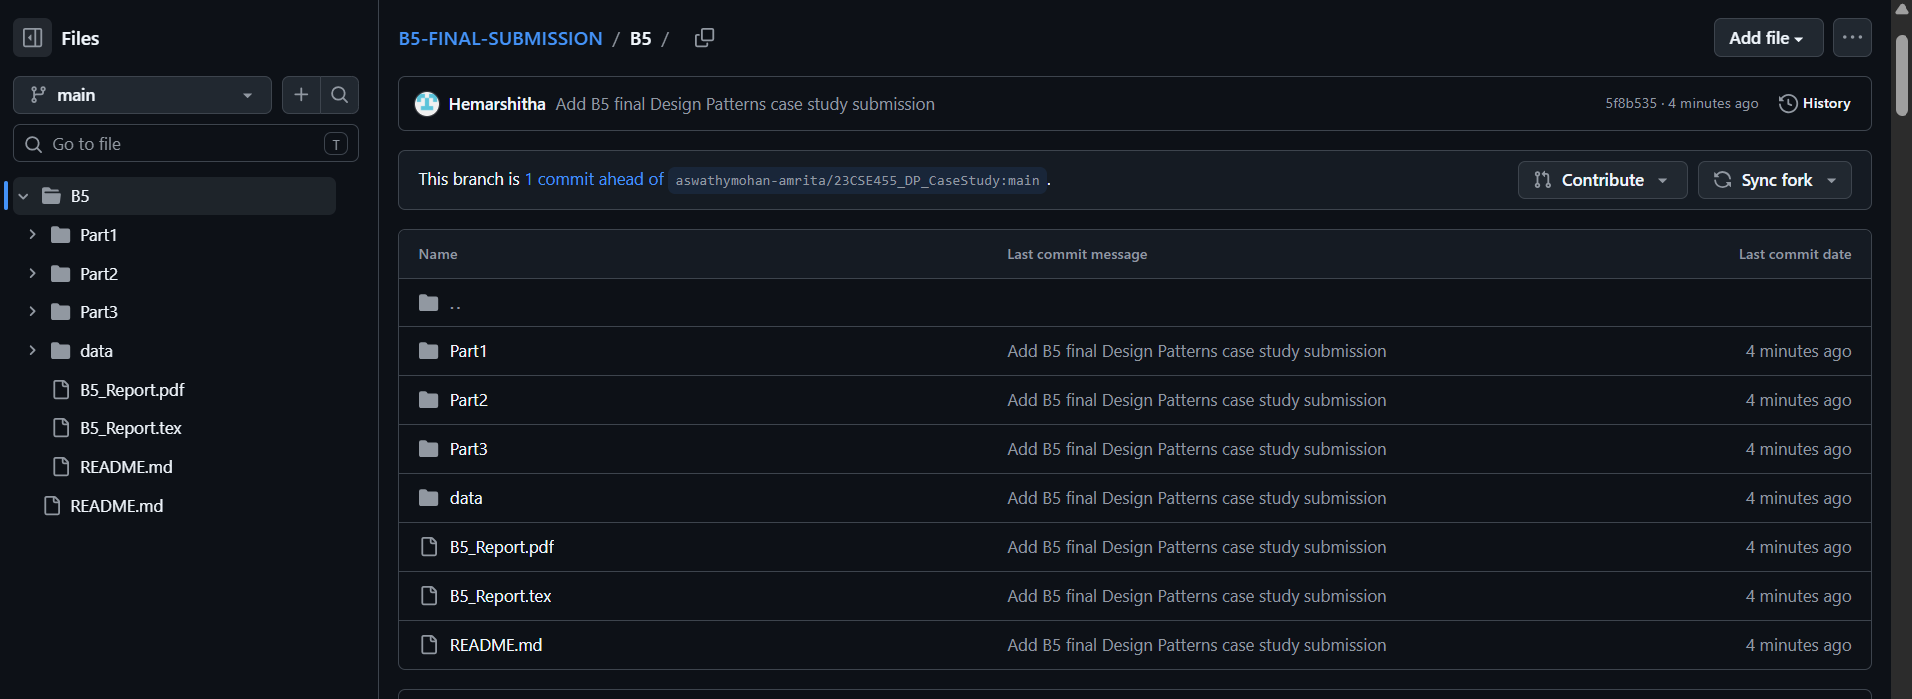
\includegraphics[width=\textwidth]{github_b5_folder.png}
    \caption{B5 team folder in the GitHub submission repository.}
    \label{fig:b5-github-folder}
\end{figure}

\section{References}
\begin{thebibliography}{9}
\bibitem{daplanstan} Geert Claes, \textit{DaPlanStan}, source repository, \url{https://github.com/GeertClaes/daplanstan}.
\bibitem{gof} E. Gamma, R. Helm, R. Johnson, J. Vlissides, \textit{Design Patterns: Elements of Reusable Object-Oriented Software}, Addison-Wesley, 1994.
\bibitem{grasp} C. Larman, \textit{Applying UML and Patterns}, Prentice Hall. GRASP responsibility-assignment patterns.
\bibitem{rails} Ruby on Rails Guides, \url{https://guides.rubyonrails.org/}.
\bibitem{ruby} Ruby language documentation, \url{https://www.ruby-lang.org/}.
\end{thebibliography}

\appendix
\section{Final Dataset Row Counts}
\begin{tabular}{lr}\toprule Dataset & Data rows\\\midrule
patterns.csv & 9\\
pattern\_counts.csv & 23\\
patterns\_evolution.csv & 45\\
cross\_language.csv & 20\\
llm.csv & 29\\\bottomrule
\end{tabular}

\section{Final Runtime Command}
The successful full-suite verification command on the team's Windows environment was:
\begin{verbatim}
set "RAILS_ENV=test" && bundle exec ruby \
  -I"C:/Ruby34-x64/lib/ruby/gems/3.4.0/gems/minitest-mock-5.27.0/lib" \
  -e "require './config/environment'; ActiveJob::Base.queue_adapter = :test; \
  load 'bin/rails'" test
\end{verbatim}

\end{document}
